%%%%%%%%%%%%%%%%%%%%%%%%%%%%%%%%%%%%%%%%%%%%%%%%%%%%%%%%%%%%%%%%%%%%%%%%%%%%%%%%%%
\begin{frame}[fragile]\frametitle{}
\begin{center}
{\Large Probability}
\end{center}
\end{frame}

%%%%%%%%%%%%%%%%%%%%%%%%%%%%%%%%%%%%%%%%%%%%%%%%%%%%%%%%%%
\begin{frame}{Why Probability?}
\begin{itemize}
\item Real life scenarios are inherently random or too complex to be completely known. 
\item If you knew every ``Physics'' aspect of motion of a dice, you could predict the outcome, deterministically.
\item However this can never be done in practice, so there is a CHANCE of something happening.
\end{itemize}
\end{frame}

%%%%%%%%%%%%%%%%%%%%%%%%%%%%%%%%%%%%%%%%%%%%%%%%%%%%%%%%%%
\begin{frame}{Probability: the Likeliness}
\begin{itemize}
\item How likely something is to happen. 
\item Many events can't be predicted with total certainty. 
\item The best we can say is how likely they are to happen, using the idea of probability. 
\item Probability is the fraction of time that outcome would occur with repeated experiments.
\end{itemize}
\end{frame}

%%%%%%%%%%%%%%%%%%%%%%%%%%%%%%%%%%%%%%%%%%%%%%%%%%%%%%%%%%
\begin{frame}{Probability: Example}
\begin{itemize}
\item Probability (event ) = Number of ways it can happen / Total number of 
outcomes 
\item Example: the chances of rolling a ``4'' with a die 
\item Number of ways it can happen: 1 (there is only 1 face with a ``4'' on it) 
\item Total number of outcomes: 6 (there are 6 faces altogether) 
 \item Probability of  this event  = 1/ 6 
\end{itemize}
\end{frame}

%%%%%%%%%%%%%%%%%%%%%%%%%%%%%%%%%%%%%%%%%%%%%%%%%%%%%%%%%%
\begin{frame}{Probability: Example}
\begin{itemize}
\item There are 5 marbles in a bag: 4 are blue, and 1 is red. 
\item What is the probability that a blue marble gets picked? 
\item Number of ways it can happen: 4 (there are 4 blues) 
\item Total number of outcomes: 5 (there are 5 marbles in total) 
 
\item Probability of  this event  = 4 / 5 
\end{itemize}
\end{frame}

%%%%%%%%%%%%%%%%%%%%%%%%%%%%%%%%%%%%%%%%%%%%%%%%%%%%%%%%%%
\begin{frame}{Probability: Example}
\begin{itemize}
\item Flip 3 coins. What is the probability that we get exactly two heads?
\item Flip 1 coin, you get either H or T. Then flip 2nd coin, draw further branches (like below)
\item At the end you will have 8 possible outcomes
\begin{center}
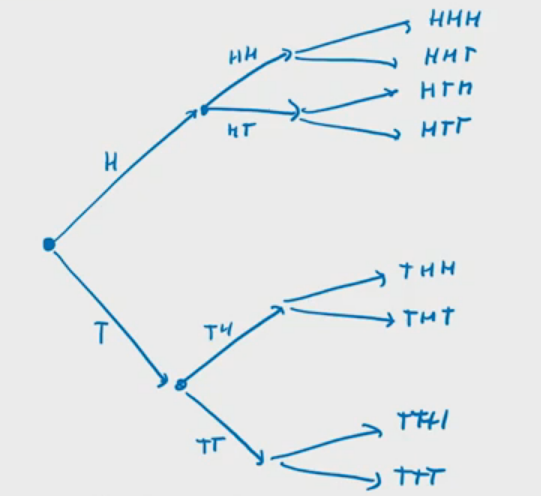
\includegraphics[width=0.5\linewidth,keepaspectratio]{math1}
\end{center}

\tiny{(Ref: Math for Machine Learning - AWS Brent Werness)}

\item What we want are HHT, HTH, THH. So 3 out of 8. 
\item Probability of  this event  = 3 / 8

\end{itemize}


\end{frame}


%%%%%%%%%%%%%%%%%%%%%%%%%%%%%%%%%%%%%%%%%%%%%%%%%%%%%%%%%%
\begin{frame}{Probability} 
\begin{definition}
Given an experiment, let $S$ be the set of all possible outcomes ($S$ is often called the \underline{sample space}) and $A$ be the event of some particular outcomes (so $A\subseteq S$).  The probability of $A$, denoted by $P(A)$, is the relative proportion of $A$ in $S$.
\end{definition}

\end{frame}

%%%%%%%%%%%%%%%%%%%%%%%%%%%%%%%%%%%%%%%%%%%%%%%%%%%%%%%%%%
\begin{frame}{Probability} 
\begin{example}
Suppose we are rolling a fair die, then $S=\{1,2,3,4,5,6\}$.  Let $A$ be the event that the outcome is an even number, that is, $A=\{2,4,6\}$.  Then $P(A)= 1/2$.
\end{example}

\begin{example}
Suppose we are rolling two fair dice, and let $A$ be the event that the sum of outcomes is either 6 or 7.  Then $P(A)= 11/35$.
\end{example}
\end{frame}

%%%%%%%%%%%%%%%%%%%%%%%%%%%%%%%%%%%%%%%%%%%%%%%%%%%%%%%%%%
\begin{frame}{Some terminologies }
\begin{itemize}
\item Experiment or Trial: an action where the result is uncertain. Example: Tossing a coin, throwing dice are examples of experiments. 
\item Outcome: A single possibility from the experiment. E.g. $\Omega = {HHT, THT, \ldots}$, each of these are outcomes.
\end{itemize}
\end{frame}

%%%%%%%%%%%%%%%%%%%%%%%%%%%%%%%%%%%%%%%%%%%%%%%%%%%%%%%%%%
\begin{frame}{Event}
\begin{itemize}
\item Event: a set of outcomes/results of an experiment 
 \item An event is what we are looking for ue $E={ExactlyTwoHeads}$. E is any subset of the sample space. The set of all events associated with a given
experiment is called the event space.
\item Example Events: 
\begin{itemize}
\item Getting a Tail when tossing a coin is an event 

\item Rolling a ''5'' is an event. 
\end{itemize}
\item An event can include one or more possible outcomes: 
\begin{itemize}
\item Choosing a ''King'' from a deck of cards (any of the 4 Kings) is an 
event 
\item Rolling an ''even number'' (2, 4 or 6) is also an event 
\end{itemize}
\end{itemize}
\end{frame}

%%%%%%%%%%%%%%%%%%%%%%%%%%%%%%%%%%%%%%%%%%%%%%%%%%%%%%%%%%
\begin{frame}
\frametitle{Sample space }
\begin{itemize}
\item  
Sample Space: all the possible outcomes of an experiment. Example: choosing a card from a deck 
\begin{itemize}
\item There are 52 cards in a deck (not including Jokers) 
\item So  the  Sample  Space  is  all  52  possible  cards:  {Ace  of  Hearts,  2  of 
Hearts, etc. } 
\end{itemize}
\item A Sample Point is just one possible outcome. 
\item And an Event can be one or more of the possible outcomes. 
\item Flipping the coin:  the sample space is  $\{H,T\}$.

\item Whats the sample space of number of heads if we flip a coin 10 times?

\item $\{0,1,\ldots,10\}$

\end{itemize}
\end{frame}

%%%%%%%%%%%%%%%%%%%%%%%%%%%%%%%%%%%%%%%%%%%%%%%%%%%%%%%%%%
\begin{frame}
\frametitle{Probability of an event? }
\begin{itemize}
\item  Both `event' and `probability' are intuitively understood by most 
people, but we need to establish certain rules. 
\item  `Rain tomorrow', `3 or fewer cyclones next year', `Crop yield will 
exceed a given threshold' are  all examples of `events' whose 
`probabilities' might be of interest. 
\end{itemize}

\begin{center}
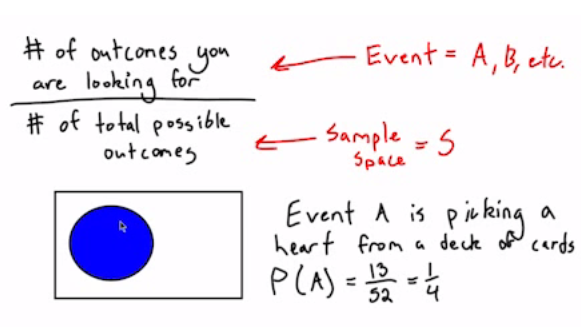
\includegraphics[width=0.65\linewidth,keepaspectratio]{evsamp}
\end{center}
\end{frame}


%%%%%%%%%%%%%%%%%%%%%%%%%%%%%%%%%%%%%%%%%%%%%%%%%%%%%%%%%%%
%\begin{frame}{Probability, continued} 
%\begin{example}
%If we choose a real number $x$ from the interval $[0,5]$, what is the probability that $2\leq x \leq 4$?  In this case, $S=[0,5]$ and $A=[2,4]$.  It follows that $P(A)= 2/5$.
%\end{example}
%
%\begin{example}
%\begin{center}
%%\includegraphics[width=3cm]{circle.png}
%\end{center}
%If we choose a point from the square above, the probability that the point belongs to the shaded region equals  $\frac{(2r)^2-\pi r^2}{(2r)^2}= 1-\frac{\pi}{4}= 0.215$.
%\end{example}
%\end{frame}

%%%%%%%%%%%%%%%%%%%%%%%%%%%%%%%%%%%%%%%%%%%%%%%%%%%%%%%%%%
\begin{frame}{Axioms* of Probability}
\begin{itemize}
\item Probability is between 0 and 1. ie $P(E) \in [0,1]$
\item Outcome is always from the sample space.
\item Summation of probabilities of all possible outcomes is 1
\end{itemize}

* Axioms are statements considered to be true without any proof.
\end{frame}



%%%%%%%%%%%%%%%%%%%%%%%%%%%%%%%%%%%%%%%%%%%%%%%%%%%%%%%%%%
\begin{frame}{Properties of Probability}
Let $S$ be the sample space and $A,B$ be events.  Then
\begin{itemize}
\item $P(S)=1, P(\emptyset)=0$. 
\item If $A\subseteq B$, then $P(A)\leq P(B)$.  In particular, $0\leq P(A)\leq 1$. 
\item $P(A\cup B)=P(A)+P(B)-P(A\cap B)$.  In particular, if $A$ and $B$ are disjoint, then $P(A
\cup B)=P(A)+P(B)$. 
\item $P(A^c)=1-P(A)$.
\end{itemize}
\end{frame}


%%%%%%%%%%%%%%%%%%%%%%%%%%%%%%%%%%%%%%%%%%%%%%%%%%%%%%%%%%
\begin{frame}
\frametitle{Visualizing Probability}
\begin{itemize}
\item  Let rectangular region being of entire sample space. Area is ``1''.
\item Points are outcomes
\item Events are collection of outcomes, so sub-regions.
\item Probability is shown as area of the sub-region.
\end{itemize}

\begin{center}
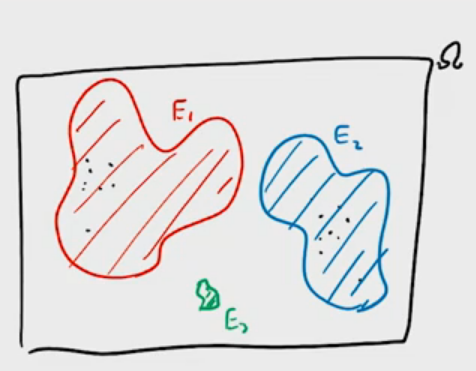
\includegraphics[width=0.5\linewidth,keepaspectratio]{math2}
\end{center}

\tiny{(Ref: Math for Machine Learning - AWS Brent Werness)}
\end{frame}

%%%%%%%%%%%%%%%%%%%%%%%%%%%%%%%%%%%%%%%%%%%%%%%%%%%%%%%%%%
\begin{frame}
\frametitle{Visualizing Probability}
\begin{itemize}
\item  Union of Events is sum of probability when they are Exclusive.
\item If they are not, meaning there is some intersection between events, then total probability is sum of both minus the intersection (as it got included twice)
\item For 3 events summation, add all 3, minus 3 double overlaps, plus add single triple overlap.
\end{itemize}

\begin{center}
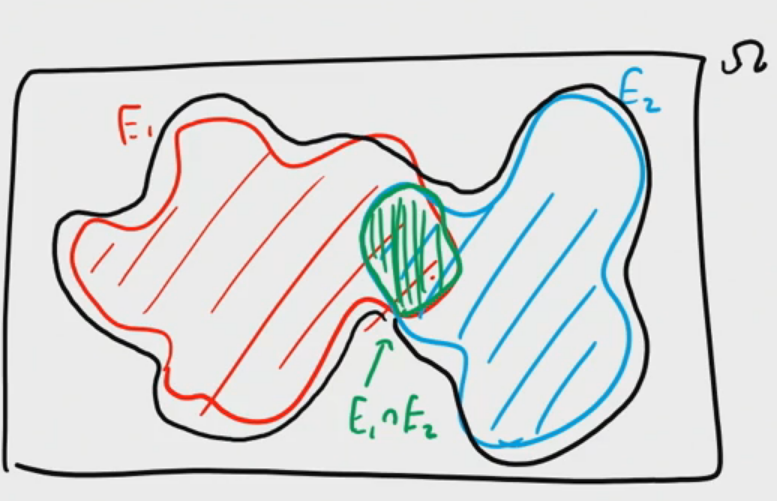
\includegraphics[width=0.5\linewidth,keepaspectratio]{math3}
\end{center}

\tiny{(Ref: Math for Machine Learning - AWS Brent Werness)}
\end{frame}



%%%%%%%%%%%%%%%%%%%%%%%%%%%%%%%%%%%%%%%%%%%%%%%%%%%%%%%%%%%%%%%%%%%%%%%%%%%%%%%%%%
\begin{frame}[fragile]\frametitle{}
\begin{center}
{\Large Probability of multiple variables}
\end{center}
\end{frame}

%%%%%%%%%%%%%%%%%%%%%%%%%%%%%%%%%%%%%%%%%%%%%%%%%%%%%%%%%%
\begin{frame}
\frametitle{Joint Probability}
\begin{itemize}
\item  To denote the probability of multiple variables AT THE SAME TIME.
\item Say, two variables, gender and hair-length.  $P(male, short)$ is the probability that a person is male and has short hair.
\end{itemize}
\end{frame}

%%%%%%%%%%%%%%%%%%%%%%%%%%%%%%%%%%%%%%%%%%%%%%%%%%%%%%%%%%
\begin{frame}
\frametitle{Conditional Probability}
\begin{itemize}
\item  To denote the probability of one event AFTER THE OTHER HAS OCCURED.
\item  $P (long hair | male)$ is the probability of having long hair given that a person is male.
\end{itemize}
\end{frame}

%%%%%%%%%%%%%%%%%%%%%%%%%%%%%%%%%%%%%%%%%%%%%%%%%%%%%%%%%%
\begin{frame}
\frametitle{Marginal Probability}
\begin{itemize}
\item  To denote the probability of one event IRRESPECTIVE OF OTHER EVENTS.
\item  Probability of person being male is given by $P(male)$. It doesn't matter whether or not the person has short hair or long.
\end{itemize}
\end{frame}

%%%%%%%%%%%%%%%%%%%%%%%%%%%%%%%%%%%%%%%%%%%%%%%%%%%%%%%%%%
\begin{frame}
\frametitle{Relation between joint, conditional and marginal probabilities}


\begin{itemize}
\item  $P(A,B) = P(B|A)P(A)$
\item $P(male,long hair)=P(long hair|male) P(male)$
\item That is, probability of a person being male and having long hair =
probability of person being male times probability of having long hair
given person is male.
\item Bayes theorem is a relation between conditional and marginal probabilities of two
variables $P(A|B) = \frac{P(B|A)P(A)}{P(B)}$
\end{itemize}
\end{frame}

%%%%%%%%%%%%%%%%%%%%%%%%%%%%%%%%%%%%%%%%%%%%%%%%%%%%%%%%%%%%%%%%%%%%%%%%%%%%%%%%%%
\begin{frame}[fragile]\frametitle{}
\begin{center}
{\Large Probability Formulation}
\end{center}
\end{frame}


%%%%%%%%%%%%%%%%%%%%%%%%%%%%%%%%%%%%%%%%%%%%%%%%%%%%%%%%%%
\begin{frame}{Unions and intersections }

\begin{itemize}
\item The union of two events A and B consists of everything included in A 
or B or both. Let  
\begin{itemize}
\item A = rain tomorrow
\item  B = rain the day after tomorrow
\item C = 3 or fewer cyclones
\item D = 4 or 5 cyclones
\end{itemize}
\item Then  
\begin{itemize}
\item $A \cup B$= rain in the next 2 days
\item $C \cup D$ = 5 or fewer cyclones
\end{itemize}
\item $ P(C \cup D) = P(C) + P(D)$, because C and D  are mutually exclusive 
(they don't overlap). 
\end{itemize}
\end{frame}

%%%%%%%%%%%%%%%%%%%%%%%%%%%%%%%%%%%%%%%%%%%%%%%%%%%%%%%%%%
\begin{frame}{Unions and intersections }

\begin{itemize}
\item $P(A \cup B) \neq P(A) + P(B)$ because A and B do overlap. 
\item$ P(A \cup B) =P(A) + P(B) - P(A \cap B)$. 
\item   $P(A \cap B)$ is the intersection of A and B; it includes everything that is in 
both A and B, and is counted twice if we add P(A) and P(B). 
\end{itemize}

\begin{center}
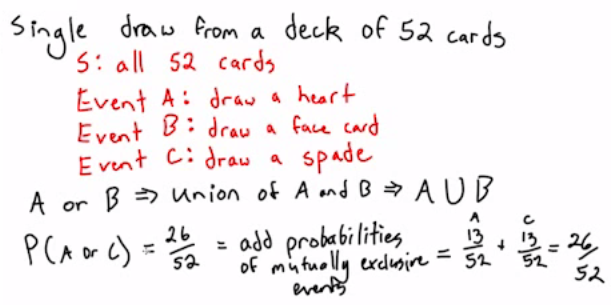
\includegraphics[width=0.65\linewidth,keepaspectratio]{undis}
\end{center}
\end{frame}

%%%%%%%%%%%%%%%%%%%%%%%%%%%%%%%%%%%%%%%%%%%%%%%%%%%%%%%%%%
\begin{frame}{Unions and intersections }
\begin{itemize}
\item In our example  
\begin{itemize}
\item $A \cap B$  = (rains tomorrow and the day after tomorrow).  
\item  $C \cap D$  is empty - it is impossible for C and D to occur 
simultaneously, so $P(C \cap D)= 0$. 
\end{itemize}

\end{itemize}
\begin{center}
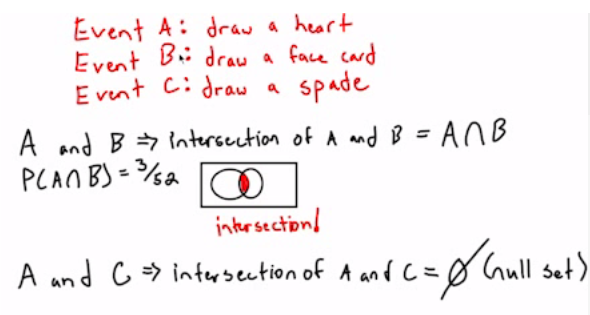
\includegraphics[width=0.65\linewidth,keepaspectratio]{intdis}
\end{center}
\end{frame}

%%%%%%%%%%%%%%%%%%%%%%%%%%%%%%%%%%%%%%%%%%%%%%%%%%%%%%%%%%
\begin{frame}{Joint Probability}

\begin{itemize}
\item Multiple events and we are trying to find chance of happening all of them together
\item So? Intersection set of all events
\item  If A and C are independent, $P(A \cup C) = P(A)P(C)$. 
%\item  If A and C are dependent, $P(A \cup C) = P(A)P(C)$. 
\end{itemize}
\end{frame}



%%%%%%%%%%%%%%%%%%%%%%%%%%%%%%%%%%%%%%%%%%%%%%%%%%%%%%%%%%
\begin{frame}{Independence }

\begin{itemize}
\item Two events are independent, if the occurrence of one does not affect the probability of occurrence of the other.
\item Similarly, two random variables are independent if the realization of one does not affect the
probability distribution of the other.
\item Example: rolling dice. First outcome, does not influence second outcome at all.
\item In pack of cards: pick a card and then pick a card again, are independent if the first card is put back.
\end{itemize}
\end{frame}

%%%%%%%%%%%%%%%%%%%%%%%%%%%%%%%%%%%%%%%%%%%%%%%%%%%%%%%%%%
\begin{frame}{Independence }
\begin{itemize}
\item In dice example  
\begin{itemize}
\item $A$  = getting 3  
\item  $B$ = getting 6
\item  $C$ = getting even number
\end{itemize}
\item Total outcome of 2 events, $6x6$ pairs of possible outcomes, e.g. 1-1, 1-2,1-3 \ldots, 6-6.
\item $P(A \cap B) = P(A)P(B) = 1/6 \times 1/6 = 1/36$. 
\item $P(A \cap C) = P(A)P(C) = 1/6 \times 3/6 = 3/36$. 
\item {\bf NOTE: A and C are not outcome of same event, which would have been NULL. They are two separate events, one after another, thus there is non-zero probability}
\end{itemize}
\end{frame}


%%%%%%%%%%%%%%%%%%%%%%%%%%%%%%%%%%%%%%%%%%%%%%%%%%%%%%%%%%
\begin{frame}{Without replacement? }
\begin{itemize}
\item First pair pulled is black
\item Second pair getting black without putting the first one back.
\item These are Dependent events. So answer is not pure multiplication, but with some adjustment.
\item Conditional Probability is for Dependent probabilities
\end{itemize}
\begin{center}
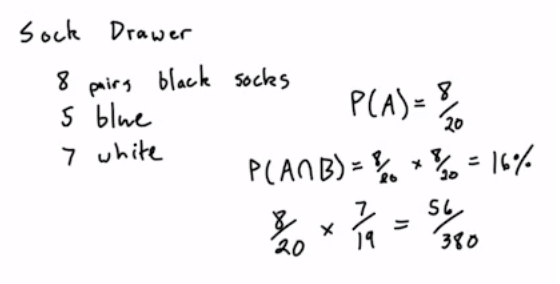
\includegraphics[width=0.65\linewidth,keepaspectratio]{socks}
\end{center}
\end{frame}

%%%%%%%%%%%%%%%%%%%%%%%%%%%%%%%%%%%%%%%%%%%%%%%%%%%%%%%%%%
\begin{frame}{Conditional probability }
\begin{center}
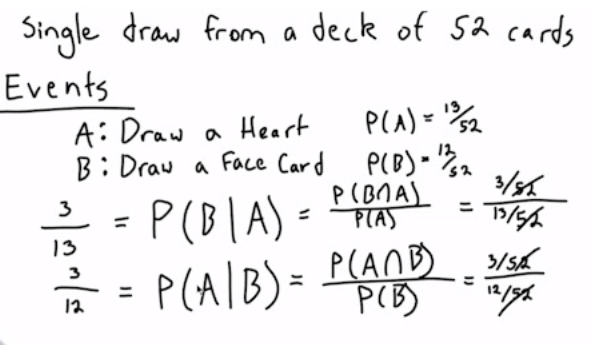
\includegraphics[width=0.5\linewidth,keepaspectratio]{condprob1}
\end{center}
\begin{itemize}
\item Calculate probabilities of A and B, independently.
\item but then if I say, that the first card is Heart, then whats the probability of Face Card.
\item There are 13 hearts. Among hearts there are 3 face cards. So, 3 /13. 3 face-heart cards, total 13 hearts.
\item reverse, first face, then whats prbability of getting heart. So, 12 face cards and 3 out of them are hearts. So, 3/12.
\end{itemize}
\end{frame}


%%%%%%%%%%%%%%%%%%%%%%%%%%%%%%%%%%%%%%%%%%%%%%%%%%%%%%%%%
\begin{frame}{ Conditional probability}

\begin{itemize}
\item  If we know that one event has occurred it may change our view of the 
probability of another event. Let  
\item  A = {rain today}, B = {rain tomorrow}.  
\item  It is likely that knowledge that A has occurred will change your view 
of the probability that B will occur. 
\item  We write $P(B|A) \neq P(B), P(B|A) = P(A \cap B)/P(A)$ denotes the 
conditional probability of B, given A.  
\end{itemize}
\begin{center}
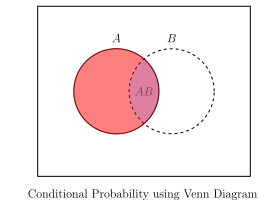
\includegraphics[width=0.3\linewidth,keepaspectratio]{condprob}
\end{center}

\end{frame}
%%%%%%%%%%%%%%%%%%%%%%%%%%%%%%%%%%%%%%%%%%%%%%%%%%%%%%%%%%
\begin{frame}

\begin{center}
\begin{tabular}{|l|l|l|l|l|}
\hline
&	A	&B	&C&	Total\\
\hline
Male&	8&	18&	13&	39\\
\hline
Female&	10	&4	&12&	26\\
\hline
Total&	18&	22&	25&	65\\
\hline
\end{tabular}
\end{center}
If one student was chosen at random, find the probability that the student got an A given that he is male.\\

\vspace{.1in}
$P(\hbox{A}|\hbox{male})=  \frac{8}{39}$  \\
\vspace{.1in}
Find the probability that a student is male given that he got an A.\\
\vspace{.1in} 
$P(\hbox{male}|\hbox{A}) =  \frac{8}{18}$ 
\end{frame}

%%%%%%%%%%%%%%%%%%%%%%%%%%%%%%%%%%%%%%%%%%%%%%%%%%%%%%%%%%
\begin{frame}
\frametitle{Conditional Probability Formula}
If events A and B are not independent, then $P(A\hbox{ and }B) = P(A) \cdot P(B | A)$.



If you pull 2 cards out of a deck, what is the probability that both are twos?\\ 
\vspace{.1in}
The probability that the first card is a two is  $\frac{4}{52}$.\\ 
\vspace{.1in}
The probability that the second card is a two, given that the first was a two, is  $\frac{3}{51}$.\\ 
\vspace{.1in}
The probability that both cards are twos is  $\frac{4}{52}\cdot \frac{3}{51}=\frac{12}{2652}\simeq 0.00452$.

\end{frame}


%%%%%%%%%%%%%%%%%%%%%%%%%%%%%%%%%%%%%%%%%%%%%%%%%%%%%%%%%%
%\begin{frame}{ Conditional probability}
%
%\begin{itemize}
%\item  Simplistically, it is just ratio of who purchased output who clicked.
%\end{itemize}
%\begin{center}
%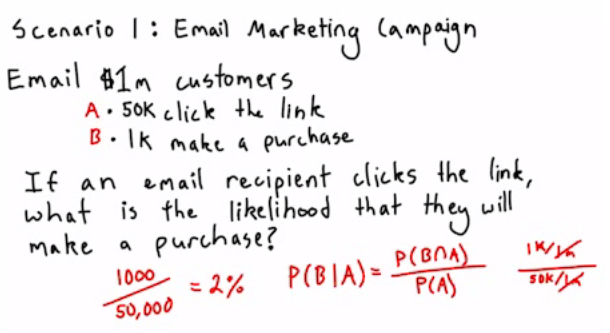
\includegraphics[width=0.5\linewidth,keepaspectratio]{condprob2}
%\end{center}
%
%%%%%%%%%%%%%%%%%%%%%%%%%%%%%%%%%%%%%%%%%%%%%%%%%%%%%%%%%
\begin{frame}{ Graphical Conditional Probability}

\begin{center}
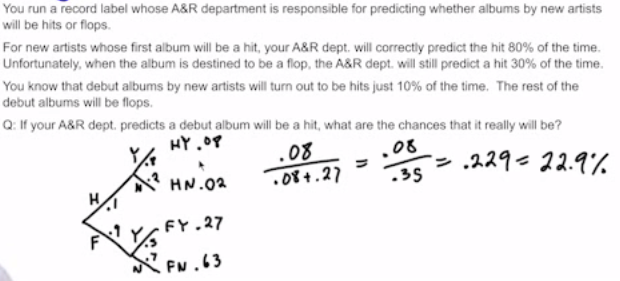
\includegraphics[width=\linewidth,keepaspectratio]{bayes1}
\end{center}
\end{frame}

%%%%%%%%%%%%%%%%%%%%%%%%%%%%%%%%%%%%%%%%%%%%%%%%%%%%%%%%%%%%%%%%%%%%%%%%%%%%%%%%%%
\begin{frame}[fragile]\frametitle{}
\begin{center}
{\Large Probability vs Likelihood}
\end{center}
\end{frame}

%%%%%%%%%%%%%%%%%%%%%%%%%%%%%%%%%%%%%%%%%%%%%%%%%%%%%%%%%%%%%%%%%%%%%%%%
\begin{frame}[fragile]\frametitle{Probability}
Lets look at Normal distribution, even though this applies for all types of distributions.


	\begin{itemize}
	\item Say, we are plotting weights (on x), frequencies on y.
	\item Probability that someones weight will be tween 32 and 34 is the area under that curve. 0.29
	\item There is 29\% chance that a randomly selected observation will have weight between 32 to 34.
	\end{itemize}

      \begin{center}
      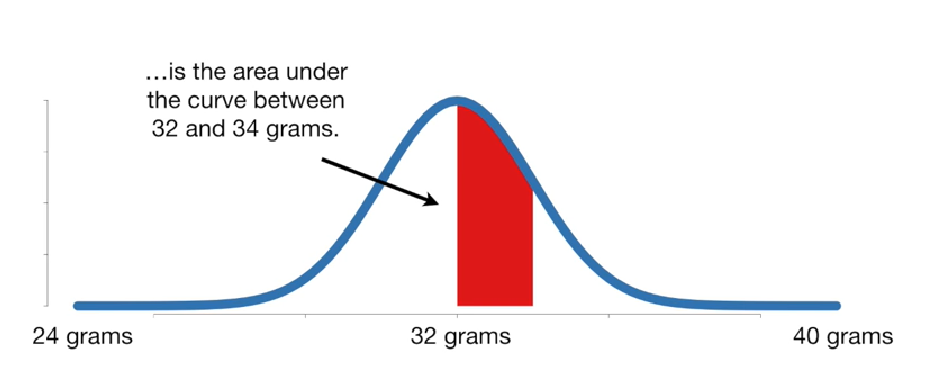
\includegraphics[width=0.8\linewidth,keepaspectratio]{statq42}
	  
	  
	  	\end{center}
		
		
\tiny{(Ref: StatQuest: Probability vs Likelihood- Josh Starmer )}

\end{frame}

%%%%%%%%%%%%%%%%%%%%%%%%%%%%%%%%%%%%%%%%%%%%%%%%%%%%%%%%%%%%%%%%%%%%%%%%
\begin{frame}[fragile]\frametitle{Likelihood}
Lets look at only one observation, say 34 grams.


	\begin{itemize}
	\item The Likelihood of the observation to have 34 is the point on this curve. 0.12
	\item If we had shifted the distribution to match mean of 32, the Likelihood would be 0.21
	\item So, Likelihoods are the y axis values for fixed data points with distributions that can be moved.
	\end{itemize}

      \begin{center}
      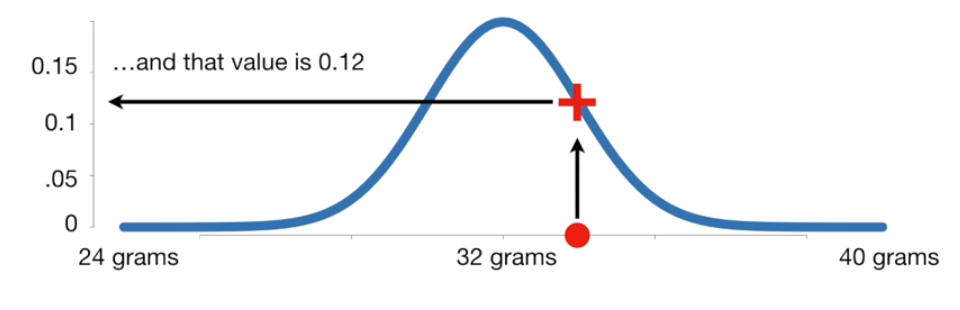
\includegraphics[width=0.5\linewidth,keepaspectratio]{statq43}
	  
	        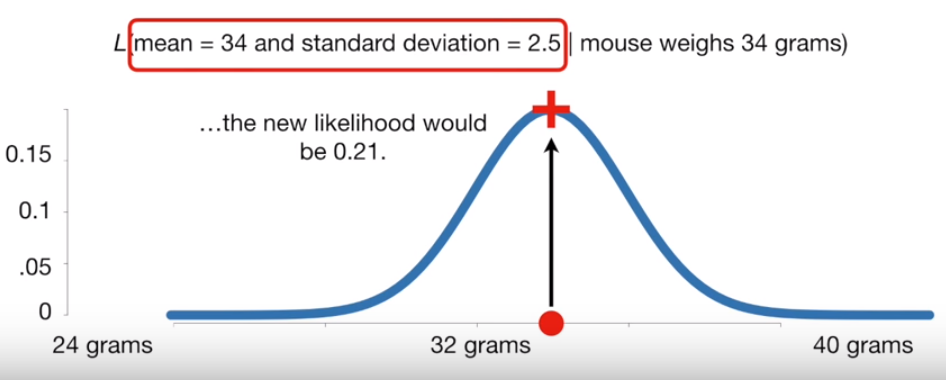
\includegraphics[width=0.5\linewidth,keepaspectratio]{statq44}
	  
	  	\end{center}

		\tiny{(Ref: StatQuest: Probability vs Likelihood- Josh Starmer )}

\end{frame}

%%%%%%%%%%%%%%%%%%%%%%%%%%%%%%%%%%%%%%%%%%%%%%%%%%%%%%%%%%%%%%%%%%%%%%%%
\begin{frame}[fragile]\frametitle{Summary}


      \begin{center}
      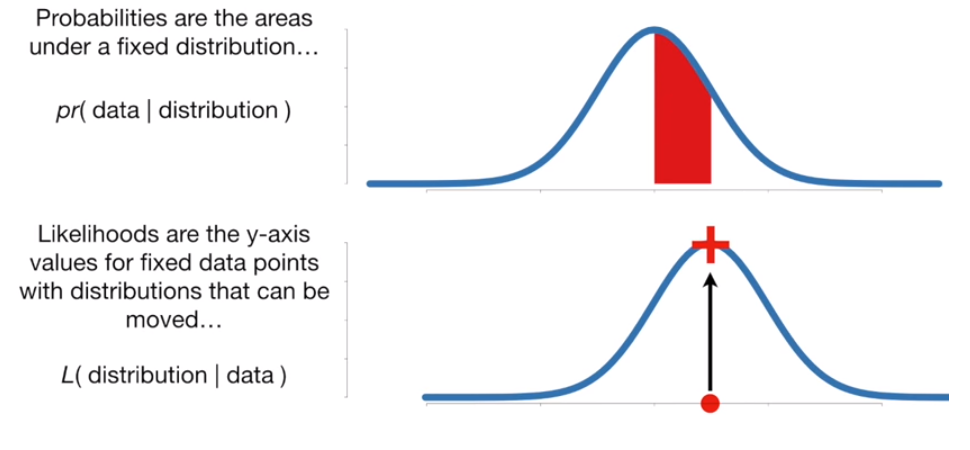
\includegraphics[width=\linewidth,keepaspectratio]{statq45}
	  
	  
	  	\end{center}

		\tiny{(Ref: StatQuest: Probability vs Likelihood- Josh Starmer )}

\end{frame}

%%%%%%%%%%%%%%%%%%%%%%%%%%%%%%%%%%%%%%%%%%%%%%%%%%%%%%%%%%%%%%%%%%%%%%%%%%%%%%%%%%
\begin{frame}[fragile]\frametitle{}
\begin{center}
{\Large Maximum Likelihood}
\end{center}
\end{frame}

%%%%%%%%%%%%%%%%%%%%%%%%%%%%%%%%%%%%%%%%%%%%%%%%%%%%%%%%%%%%%%%%%%%%%%%%
\begin{frame}[fragile]\frametitle{Maximum Likelihood}
Lets say we are measuring weights \ldots

	\begin{itemize}
	\item The goal of Maximum Likelihood is to find the optimal way to fit a distribution to the data.
	\item Is the shown Normal distribution fitting the data? It is not.
	\item Likelihood of observations is away from the center of the distribution.
	\end{itemize}

      \begin{center}
      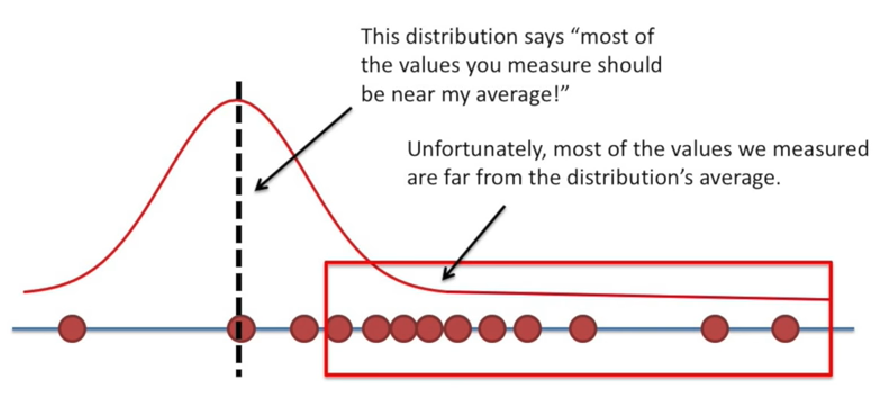
\includegraphics[width=0.8\linewidth,keepaspectratio]{statq46}
	  
	  	\end{center}

		\tiny{(Ref: StatQuest: Maximum Likelihood, clearly explained!!! - Josh Starmer )}

\end{frame}

%%%%%%%%%%%%%%%%%%%%%%%%%%%%%%%%%%%%%%%%%%%%%%%%%%%%%%%%%%%%%%%%%%%%%%%%
\begin{frame}[fragile]\frametitle{Maximum Likelihood}
What if we shift the normal distribution on right so that the mean was the same as the average weight?

	\begin{itemize}
	\item The goal of Maximum Likelihood is to find the optimal way to fit a distribution to the data.
	\item Is the shown Normal distribution fitting the data? It is not.
	\item Likelihood of observations is away from the center of the distribution. Looks good.
	\item If we had shifted too much on the right, not good, again.
	\end{itemize}

      \begin{center}
      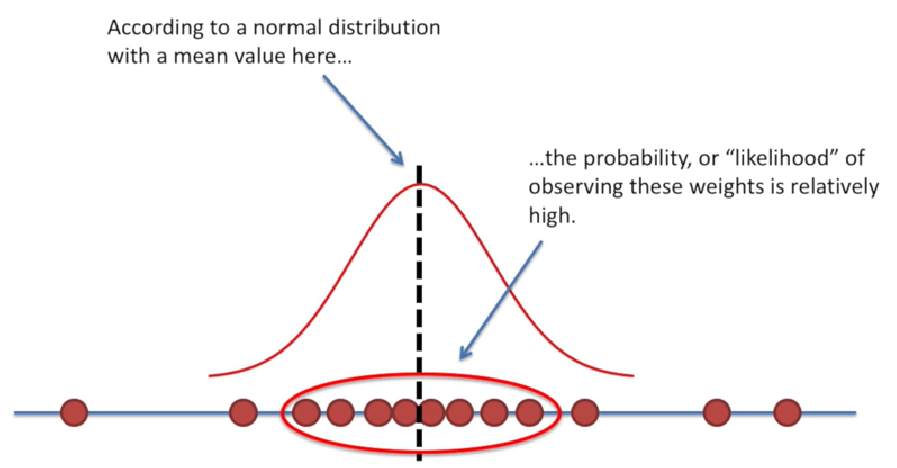
\includegraphics[width=0.6\linewidth,keepaspectratio]{statq47}
	  
	  	\end{center}

		\tiny{(Ref: StatQuest: Maximum Likelihood, clearly explained!!! - Josh Starmer )}

\end{frame}

%%%%%%%%%%%%%%%%%%%%%%%%%%%%%%%%%%%%%%%%%%%%%%%%%%%%%%%%%%%%%%%%%%%%%%%%
\begin{frame}[fragile]\frametitle{Maximum Likelihood}
We plot all the possible shifting positions and find the best!!


      \begin{center}
      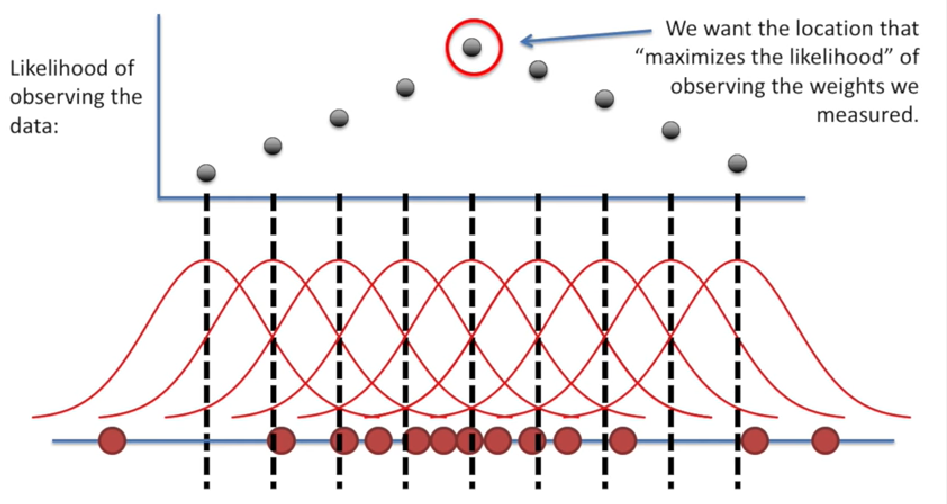
\includegraphics[width=0.8\linewidth,keepaspectratio]{statq48}
	  
	  	\end{center}

		\tiny{(Ref: StatQuest: Maximum Likelihood, clearly explained!!! - Josh Starmer )}

\end{frame}

%%%%%%%%%%%%%%%%%%%%%%%%%%%%%%%%%%%%%%%%%%%%%%%%%%%%%%%%%%%%%%%%%%%%%%%%
\begin{frame}[fragile]\frametitle{Maximum Likelihood}
Results:

      \begin{center}
      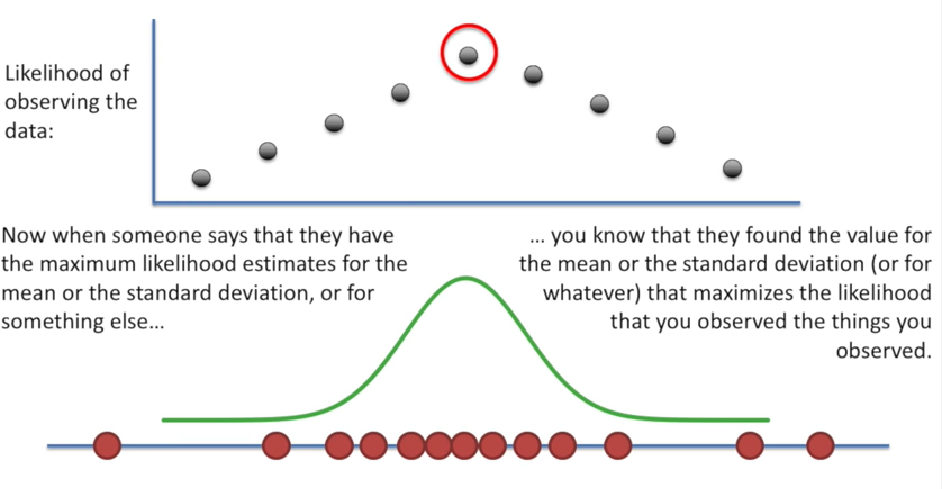
\includegraphics[width=0.8\linewidth,keepaspectratio]{statq50}
	  
	  	\end{center}

		\tiny{(Ref: StatQuest: Maximum Likelihood, clearly explained!!! - Josh Starmer )}

\end{frame}
